\mychapter{Acompanhamento de acesso de estudantes no Moodle}\label{ch:apendice}

Este apêndice relata uma experiência realizada na disciplina de Processamento da Informação (CS1) na UFABC no primeiro quadrimestre de 2024, em duas turmas. A motivação foi substituir a lista de presença por um processo automático que verifica o acesso dos estudantes no ambiente Moodle durante as aulas realizadas no laboratório. Para isso, foi desenvolvido o serviço chamado \texttt{LabMoodle}, que acompanha as atividades dos estudantes cadastrados em uma disciplina no Sistema de Gerenciamento de Aprendizagem Moodle, disponibilizado em \url{http://mctest.ufabc.edu.br:8000/LabMoodle}.

Apesar de este conteúdo do apêndice não estar diretamente relacionado ao MCTest, há uma relação indireta, pois foram oferecidos 80 Exercícios de Programação (EPs) estáticos com correção automática pelo VPL (\textit{Virtual Programming Lab for Moodle}) \cite{rodriguez2012virtual}. Os exames foram gerados pelo MCTest, com correção automática também utilizando o VPL, conforme relatado no Capítulo \ref{ch:examesQT_VPL} -- \nameref{ch:examesQT_VPL}.

\section{Contexto da oferta}

A disciplina de Processamento da Informação é obrigatória para estudantes em diversos programas de nossa universidade, com uma média de 2000 matrículas por ano. A partir de 2023, a disciplina é oferecida integralmente por um único professor em um laboratório de informática. O curso tem duração de 12 semanas, com quatro horas de aula por semana. No início de 2024, foi realizado um experimento em duas turmas, A e B, com 38 e 35 estudantes matriculados, respectivamente, de fevereiro a maio. O professor ministrou aulas laboratoriais síncronas aos estudantes por meio de um projetor, apresentando \href{https://colab.research.google.com}{Google Colabs} contendo conceitos, exemplos e exercícios, conforme relatado em \citeonline{2021:Zampirolli.Teubl.ea}. Além disso, o professor disponibilizou 80 exercícios com correção automática detalhados a seguir. Também foram disponibilizadas aulas gravadas, criadas durante a pandemia de Covid-19.



\section{Intervenção pedagógica}


A disciplina aborda os conceitos fundamentais de Lógica de Programação, tal como apresentados no livro-texto de \citeonline{2017:Neves.Zampirolli}. A primeira parte do curso abrange os quatro primeiros capítulos: introdução e programas sequenciais, organização de código, condicionais e repetição. Na quinta semana, foi realizada uma revisão com um simulado utilizando uma prova antiga e o Exame 1. Nas semanas seis a dez, os capítulos cinco e seis do livro foram abordados, tratando de vetores e matrizes, respectivamente. A semana onze foi dedicada à revisão, também com um simulado utilizando uma prova antiga, e em seguida um exame final, seguido pelo exame de recuperação na semana doze. Todos esses exames são elaborados no MCTest e compostos por duas questões cada, com correção automática utilizando o \textit{plugin} VPL do Moodle.

A estratégia de ensino foi implementada com uma abordagem conceitual no Google Colab no início de cada aula, seguida pela apresentação dos Exercícios Programados (EPs), permitindo tempo para os estudantes tentarem resolvê-los. O professor então discutiu algumas soluções dos estudantes (com autorização prévia). Foram distribuídos 80 EPs ao longo dos seis capítulos do livro, com ênfase em vetores (25 EPs) e matrizes (23 EPs). Além disso, foram realizados seis testes adaptativos, correspondentes aos capítulos do livro, contendo cinco questões de múltipla escolha em papel, com correção automática, também administrados no MCTest, conforme detalhado na Seção \ref{sec:testeAdaptativo} -- \nameref{sec:testeAdaptativo}. Os EPs não foram pontuados, enquanto os testes concederam um bônus de 5\% na nota final pela participação, independentemente do desempenho obtido.

A estratégia de avaliação para este curso consistiu no Exame 1 (40\% da nota final), contendo exercícios semelhantes aos EPs. O exame final (60\% da nota final) abrangeu os tópicos da segunda parte da disciplina. Ambos os exames, inicial e final, tiveram duração de duas horas e foram realizados utilizando o navegador \textit{Safe Exam Browser} (\href{safeexambrowser.org}{SEB}), sem consulta externa. Cada questão do exame foi elaborada de forma parametrizada, com 10 casos de testes gerados automaticamente pelo MCTest. Foram geradas 40 variações para cada exame, garantindo que cada estudante recebesse uma versão única, conforme detalhado no Capítulo \ref{ch:examesQT_VPL} -- \nameref{ch:examesQT_VPL}.


\section{O Serviço \texttt{LabMoodle}}

O serviço disponibilizado em \url{http://mctest.ufabc.edu.br:8000/LabMoodle} para acompanhamento das atividades realizadas pelos estudantes no Moodle foi elaborado em PHP para a interface do professor, enquanto a lógica no servidor para a geração dos relatórios foi realizada na linguagem Python, utilizando principalmente as bibliotecas \href{https://pandas.pydata.org}{Pandas} e \href{https://seaborn.pydata.org}{Seaborn}.

O acompanhamento das atividades dos estudantes no Moodle é facilitado por meio de arquivos gerados nesse serviço. Um exemplo pode ser visto na pasta \href{http://mctest.ufabc.edu.br:8000/LabMoodle/modelos/report}{``report''}. Para obter esses arquivos, primeiramente é necessário fazer \textit{login} no Moodle e baixar o \textit{log} da disciplina em formato CSV. Em seguida, no \href{https://sig.ufabc.edu.br/sigaa/verTelaLogin.do}{SIGAA}, acessa-se o portal docente, seleciona-se a turma desejada e, dentro do menu de estudantes, é possível lançar notas e faltas e exportar uma planilha em formato XLS contendo a lista dos estudantes, ver Figura \ref{fig:ApeA_parte1}.

\begin{figure}[!ht]
    \centering
    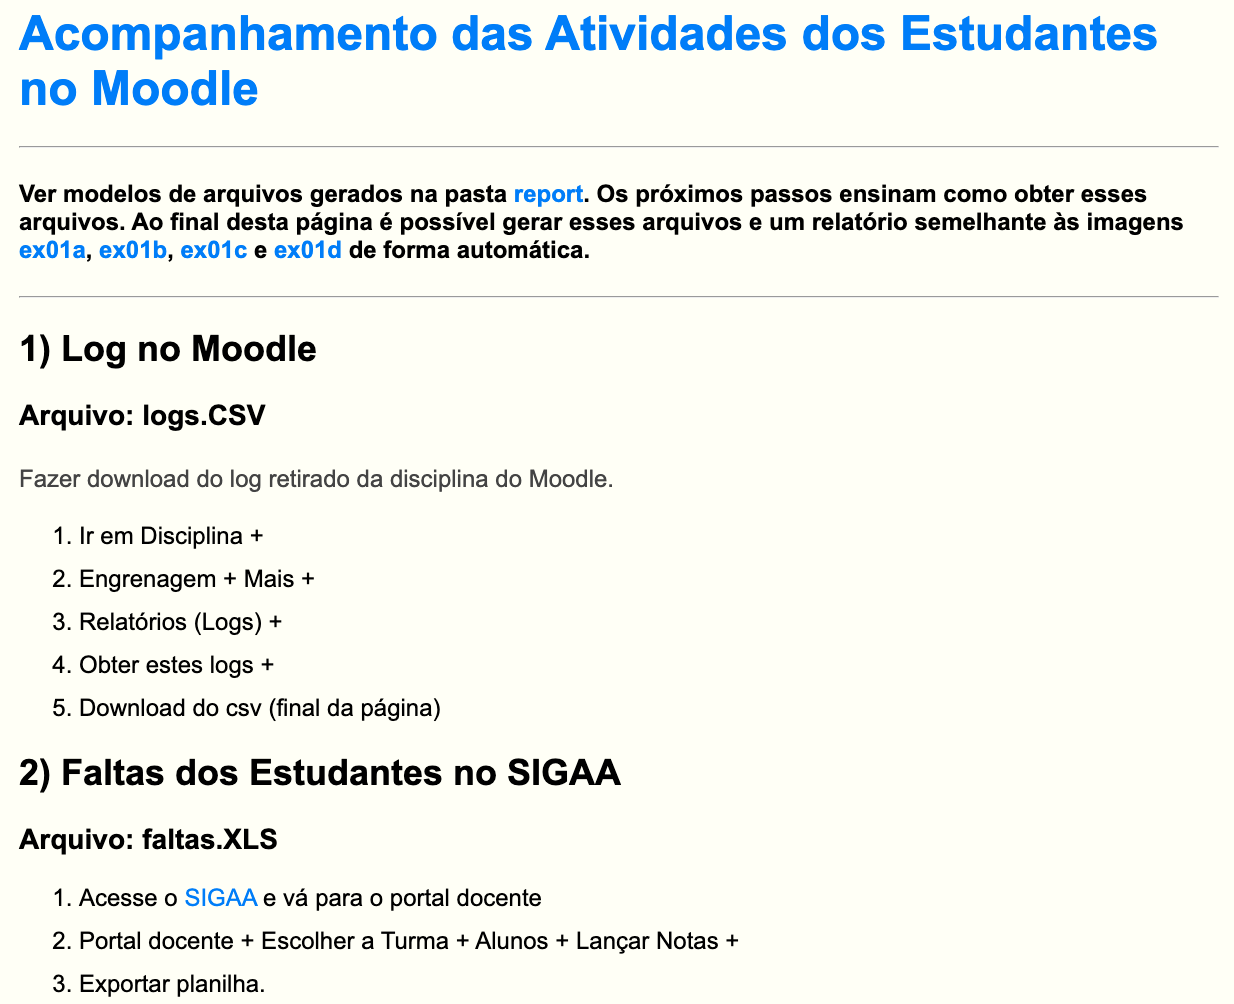
\includegraphics[width=0.9\textwidth]{ApeA_parte1.png}
     \caption{Tela do serviço - Parte 1 - informações gerais.}
  \label{fig:ApeA_parte1}
  \end{figure}


Para configurar corretamente as informações da disciplina, é necessário definir a data de início do curso como 05/02/2024 e a data de término como 07/05/2024. Além disso, é preciso filtrar o \textit{log} do Moodle pelo componente, ou deixar o valor padrão ``Tudo'', indicando que não será realizado filtro do componente. Estabelecer o número mínimo de faltas após o término do curso como 14. Para os estudantes reprovados por falta, com o conceito ``O'', deve ser marcado o \textit{checkbox} correspondente. Existe também um \textit{checkbox} para ser marcado se desejar omitir dados de estudantes. Finalmente, os dados de cada aula devem ser preenchidos: como o dia da semana, o horário de início, a duração de 2 horas, e o prefixo dos IPs do laboratório, como ``172.17.14'', conforme apresentado na Figura \ref{fig:ApeA_parte2}.


  \begin{figure}[!ht]
    \centering
    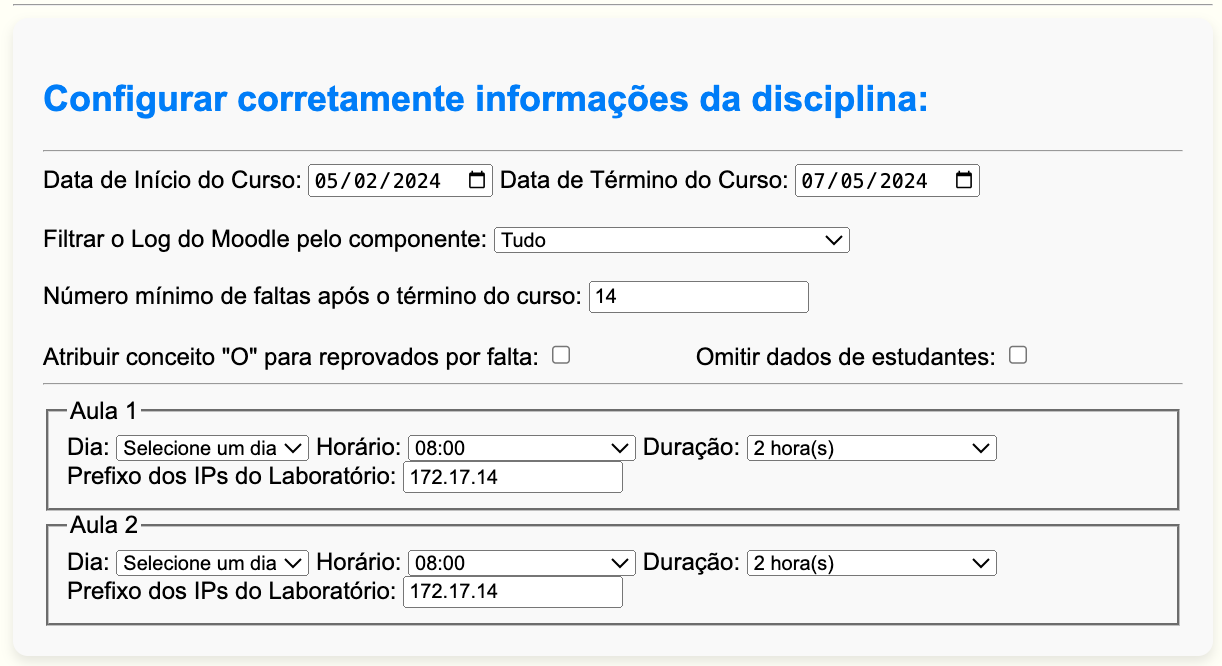
\includegraphics[width=0.9\textwidth]{ApeA_parte2.png}
     \caption{Tela do serviço - Parte 2: Configurações dos relatórios e dos dados da disciplina.}
  \label{fig:ApeA_parte2}
  \end{figure}

Finalmente, no serviço fornecido, há um formulário para realizar o \textit{upload} de arquivos a fim de gerar relatórios. Os professores são instruídos a selecionar os arquivos nos formatos CSV e XLS obtidos nos passos anteriores. Em seguida, podem escolher o botão ``Enviar'' para iniciar o processo de \textit{upload} e geração de relatório. Além disso, é fornecido um \textit{link} para visitar o projeto no \href{https://github.com/fzampirolli/LabMoodle}{GitHub}, conforme apresentado na Figura \ref{fig:ApeA_parte3}.

\begin{figure}[!ht]
\centering
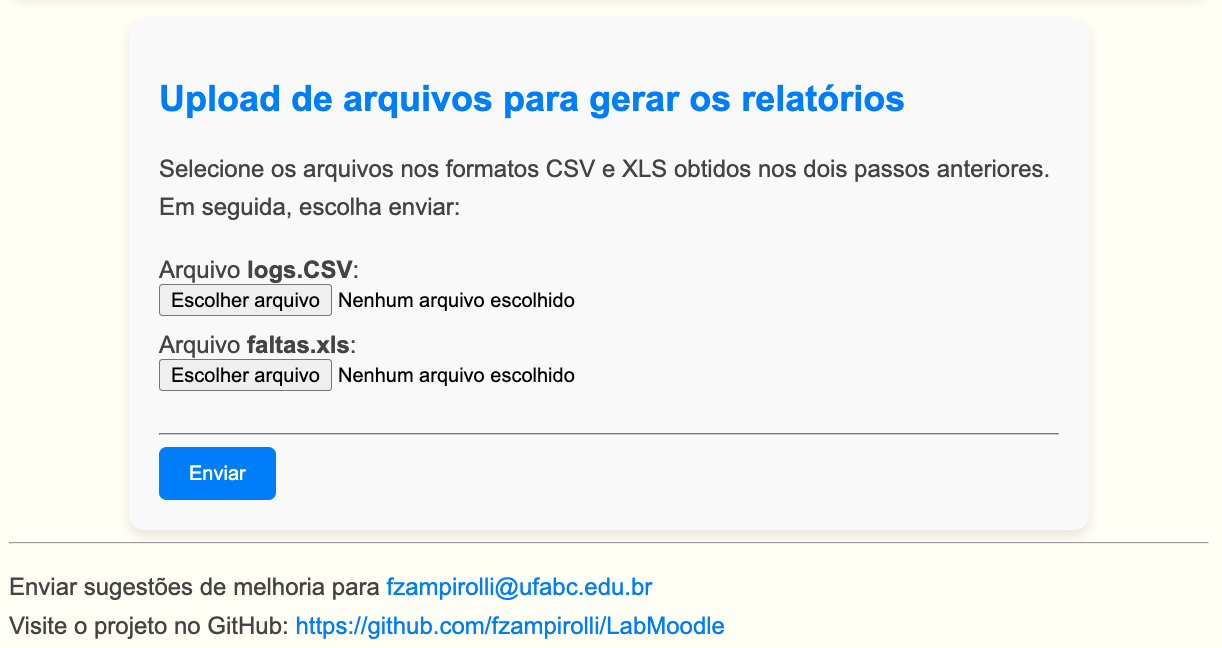
\includegraphics[width=0.9\textwidth]{ApeA_parte3.png}
    \caption{Tela do serviço - Parte 3: envio dos arquivos e geração do relatório.}
\label{fig:ApeA_parte3}
\end{figure}

O processo de geração de relatório é demorado e depende da conexão de internet. Por exemplo, demorou 2 minutos para um arquivo de \textit{log} de 45MB e gerou uma página, cujo início é apresentado na Figura \ref{fig:ApeA_relato1}. Os dados dos estudantes foram omitidos nas figuras apresentadas neste apêndice. O restante da página apresenta seis imagens e será detalhado na próxima seção de resultados e discussões.

\begin{figure}[]
\centering
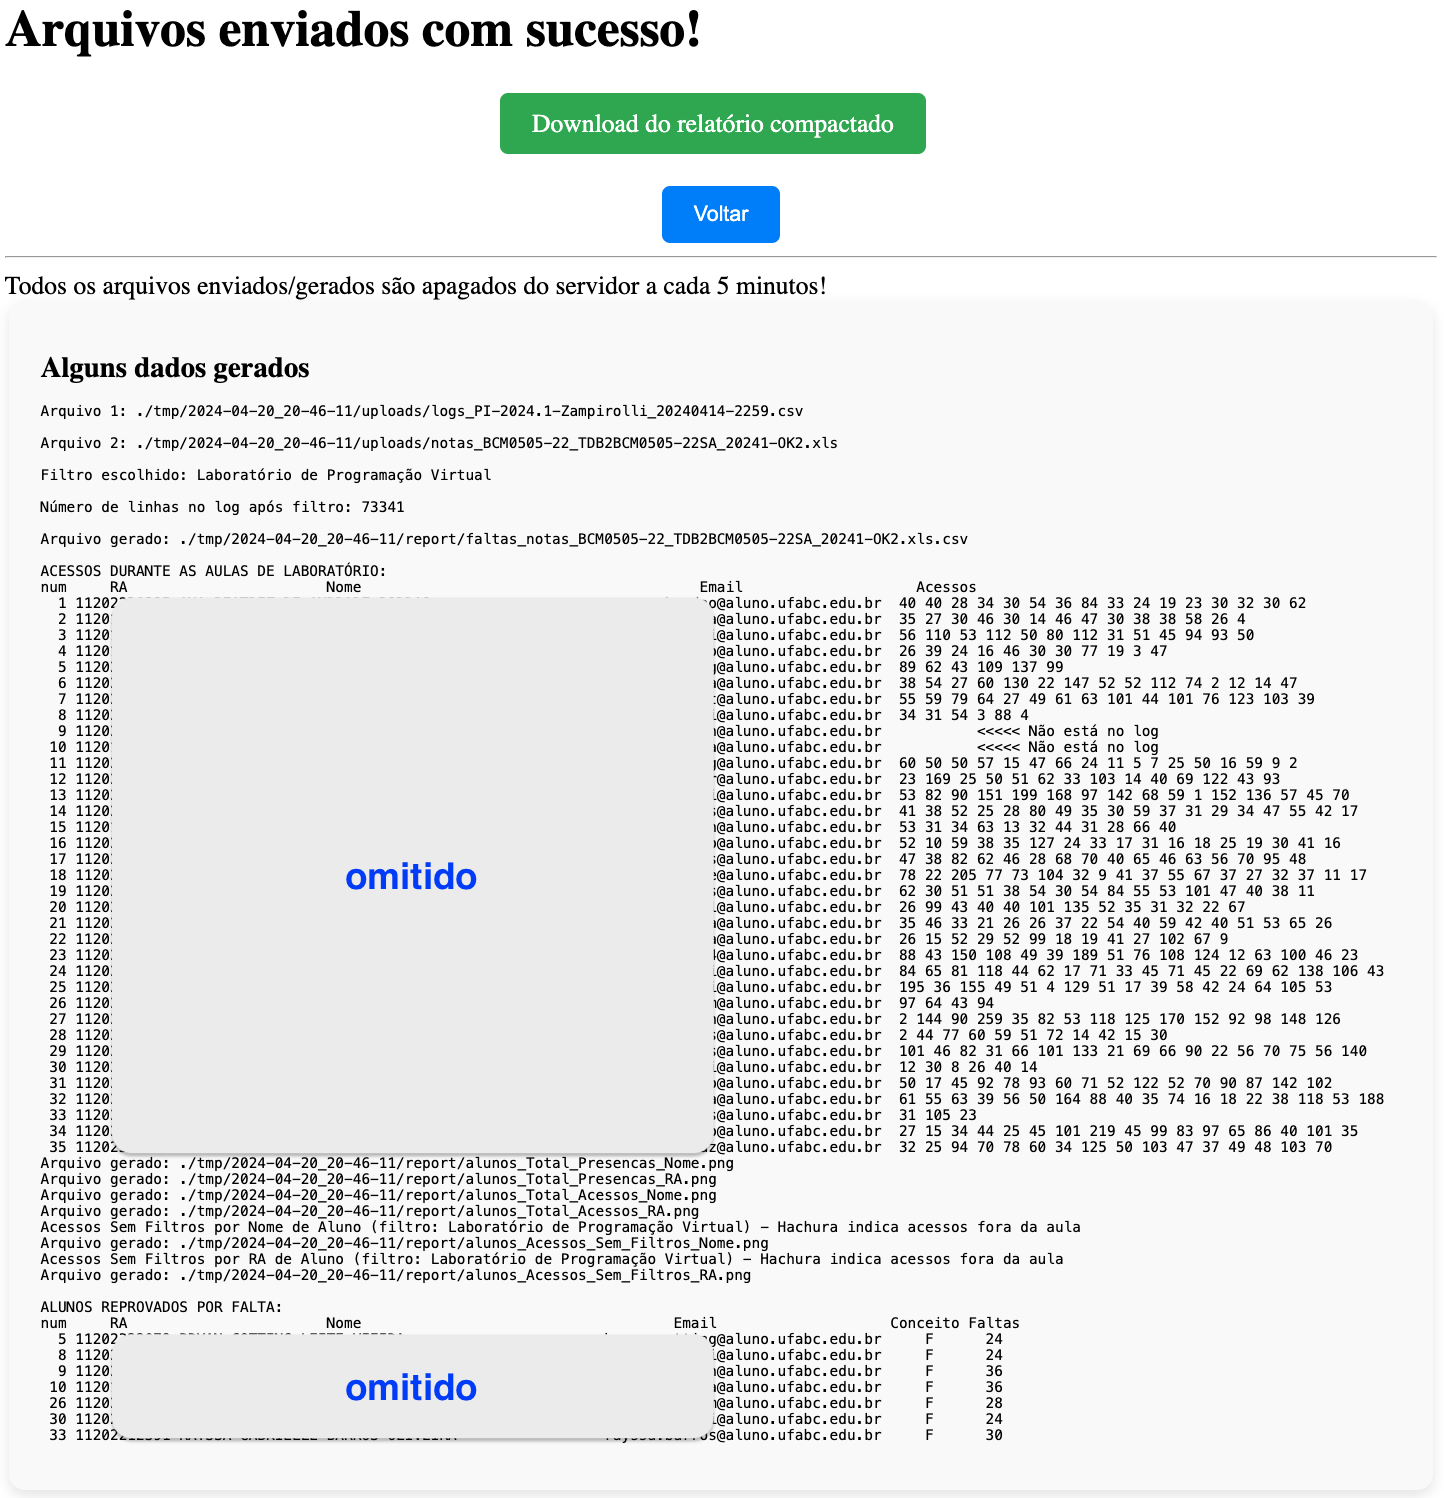
\includegraphics[width=0.99\textwidth]{ApeA_relato1.png}
    \caption{Tela do serviço - Parte inicial do relatório gerado.}
\label{fig:ApeA_relato1}
\end{figure}

Conforme ilustrado na Figura \ref{fig:ApeA_relato1}, após o envio bem-sucedido dos arquivos, o professor é informado sobre a conclusão do processo e são apresentadas algumas informações relevantes. Ele tem a opção de baixar o relatório compactado, voltar para a página anterior ou visualizar os dados gerados. Além disso, é destacado que todos os arquivos enviados ou gerados são apagados do servidor a cada 5 minutos. Os professores podem observar detalhes sobre os arquivos enviados, como seus nomes e caminhos, bem como informações sobre o filtro escolhido e o número de linhas no \textit{log} após o filtro. Também são exibidas algumas imagens geradas, como gráficos relacionados aos acessos durante as aulas de laboratório, aos estudantes reprovados por falta e aos acessos sem filtros por nome ou RA de estudante, evidenciando a presença ou ausência nas aulas. 

Destaco na Figura \ref{fig:ApeA_relato1} que nas linhas 9 e 10, dois estudantes apresentam a informação ``\verb|<<< Não está no log|'' abaixo da coluna ``Acessos''. Tal indicação sugere que esses estudantes estão registrados no sistema acadêmico SIGAA, porém não participaram de nenhuma das aulas de laboratório.

\section{Resultados e discussões}\label{sec:apendice_resultados}

Esta seção complementa a parte inicial apresentada na Figura \ref{fig:ApeA_relato1}, descrevendo os arquivos adicionais que compõem o conjunto de informações recebidas pelo professor. Junto com o relatório inicial, o professor também recebe um arquivo compactado contendo diversos outros arquivos gerados durante o processo de análise e geração de dados. Nesta seção, serão detalhados esses arquivos.

As imagens \verb|*_Nome.png| na listagem a seguir apresentam os nomes dos estudantes no eixo $x$ do gráfico, enquanto as imagens \verb|*_RA.png| mostram os números de matrícula (RA) dos estudantes. Caso o professor deseje enviar aos estudantes seus desempenhos em comparação com a turma, os gráficos com os RAs são mais apropriados. Sem redundância, nesta seção serão apresentados apenas os gráficos com RA contidos nos arquivos \verb|alunos_Acessos_Sem_Filtros_RA.png| e \verb|alunos_Total_Presencas_RA.png|, pois \verb|alunos_Total_Acessos_RA.png| pode ser visualizado no primeiro caso.
\
\begin{myboxCode}{corCSV}{\textbf{Arquivos descompactados}}\vspace{3mm}
\hrule
\begin{verbatim}
alunos_Acessos_Sem_Filtros_Nome.png
alunos_Acessos_Sem_Filtros_RA.png
alunos_Total_Acessos_Nome.png
alunos_Total_Acessos_RA.png
alunos_Total_Presencas_Nome.png
alunos_Total_Presencas_RA.png
data.json
dias_notas_BCM0505-B-22SA_20241-OK2.xls.csv
faltas_notas_BCM0505-B-22SA_20241-OK2.xls.csv
presenca_notas_BCM0505-B-22SA_20241-OK2.xls.csv
\end{verbatim}
\end{myboxCode}


\subsection{Arquivo \texttt{data.json}}

Nessa lista de arquivos possui também texto nos formatos JSON e CSV. O promeiro \verb|data.json| é apresentado um exemplo a seguir. Esse arquivo contém informações sobre o período de análise (de 5 de fevereiro a 7 de maio de 2024), o filtro aplicado (Laboratório de Programação Virtual), e detalhes sobre as aulas, incluindo dias, horas e duração. Também são fornecidos caminhos para os diretórios de \textit{upload} e relatório, bem como os arquivos CSV e XLS utilizados no processo.


\begin{myboxCode}{corCSV}{\textbf{Arquivo \texttt{data.json}}}\vspace{3mm}
\hrule
\begin{verbatim}
{
"startDate": "2024-02-05",
"endDate": "2024-05-07",
"filter_field": "Laboratório de Programação Virtual",
"min_absences": "14",
"assign_O": "off",
"omit_data": "off",
"uploadDir": ".\/tmp\/2024-04-20_20-30-22\/uploads\/",
"reportDir": ".\/tmp\/2024-04-20_20-30-22\/report\/",
"csvPath": ".\/tmp\/2024-04-20_20-30-22\/uploads\/logs_PI-2024.1-Zampirolli.csv",
"xlsPath": ".\/tmp\/2024-04-20_20-30-22\/uploads\/notas_BCM0505-B-22SA_20241-OK2.xls",
"classes": [{
        "day": "1",
        "hour": "10:00",
        "duration": "2:00",
        "ipPrefix": "172.17.14" },{
        "day": "3",
        "hour": "8:00",
        "duration": "2:00",
        "ipPrefix": "172.17.14" }]}
\end{verbatim}
\end{myboxCode}

\subsection{Arquivo \texttt{dias\_notas\_*.csv}}

O arquivo \texttt{dias\_notas\_*.csv} contém informações sobre o início e o fim de cada sessão de aula, juntamente com um prefixo de endereço IP correspondente. Cada linha representa uma sessão de aula, com as colunas representando a data e horário de início, data e horário de fim, e o prefixo do endereço IP do laboratório onde a aula ocorreu.

\begin{myboxCode}{corCSV}{\textbf{Arquivo \texttt{dias\_notas\_*.csv}}}\vspace{3mm}
    \hrule
    \begin{verbatim}
Inicio           Fim              IP
06/02/2024 10:00 06/02/2024 12:00 172.17.14
08/02/2024 08:00 08/02/2024 10:00 172.17.14
13/02/2024 10:00 13/02/2024 12:00 172.17.14
...
\end{verbatim}
\end{myboxCode}

\subsection{Arquivo \texttt{faltas\_notas\_*.csv}}

O arquivo \texttt{faltas\_notas\_*.csv} contém informações sobre os estudantes, como suas matrículas, nomes, e-mails, resultados obtidos, quantidade de faltas e situação atual. Esses dados podem ser utilizados pelo professor para atualizar o arquivo original XLS exportado do SIGAA, permitindo a atualização das colunas de Resultado e Faltas. Posteriormente, o professor pode importar essas atualizações para o sistema acadêmico, garantindo a precisão dos conceitos dos estudantes registrados.

\begin{myboxCode}{corCSV}{\textbf{Arquivo \texttt{faltas\_notas\_*.csv}}}\vspace{3mm}
\hrule
\begin{verbatim}
Matrícula Nome    E-mail                     Resultado Faltas Sit.
omitido   omitido omitido@aluno.ufabc.edu.br B          4     APR
omitido   omitido omitido@aluno.ufabc.edu.br A          8     APR
omitido   omitido omitido@aluno.ufabc.edu.br D         10     APR     
...
\end{verbatim}
\end{myboxCode}

\subsection{Arquivo \texttt{presenca\_notas\_*.csv}}

O arquivo \texttt{presenca\_notas\_*.csv} mantém as três primeiras colunas para matrículas, nomes e e-mails. Em seguida, cada coluna representa um dia de aula conforme definido pelo arquivo \texttt{dias\_notas\_*.csv}. Além disso, o arquivo inclui as colunas ``Acessos\_Sem\_Filtros'', ``Total\_Presencas'', ``Faltas'' e ``Conceito''. Esses dados são obtidos cruzando as informações dos arquivos CSV e XLS enviados pelo professor, além dos dados informados no formulário HTML antes do envio. Com base nesse arquivo \texttt{presenca\_notas\_*.csv}, foram geradas seis imagens PNG, como detalhado na próxima seção.

\begin{myboxCode}{corCSV}{\textbf{Arquivo \texttt{presenca\_notas\_*.csv}}}\vspace{3mm}
\hrule
\begin{verbatim}
... 01-06/02 02-08/02 03-13/02 ... Acessos_Sem_Filtros Total_Presencas Faltas Conceito
    40       40                     909                32               4     B
    35       27       30            767                28               8     A
                                   1433	               26              10     D
...
\end{verbatim}
\end{myboxCode}

% \subsection{Presença em aula}

% A Figura \ref{fig:ApeA_alunos_Total_Presencas_RA} mostra a imagem \verb|alunos_Total_Presencas_RA.png|, que exibe o total de presenças durante as aulas de laboratório para a turma B. A linha tracejada vermelha indica o número mínimo de faltas que um estudante pode ter sem reprovação por faltas. Um gráfico semelhante para a turma A é apresentado na Figura \ref{fig:ApeA_alunos_Total_Presencas_RA_Turma_A}.

% \begin{figure}[!ht]
%     \centering
%     \rotatebox{270}{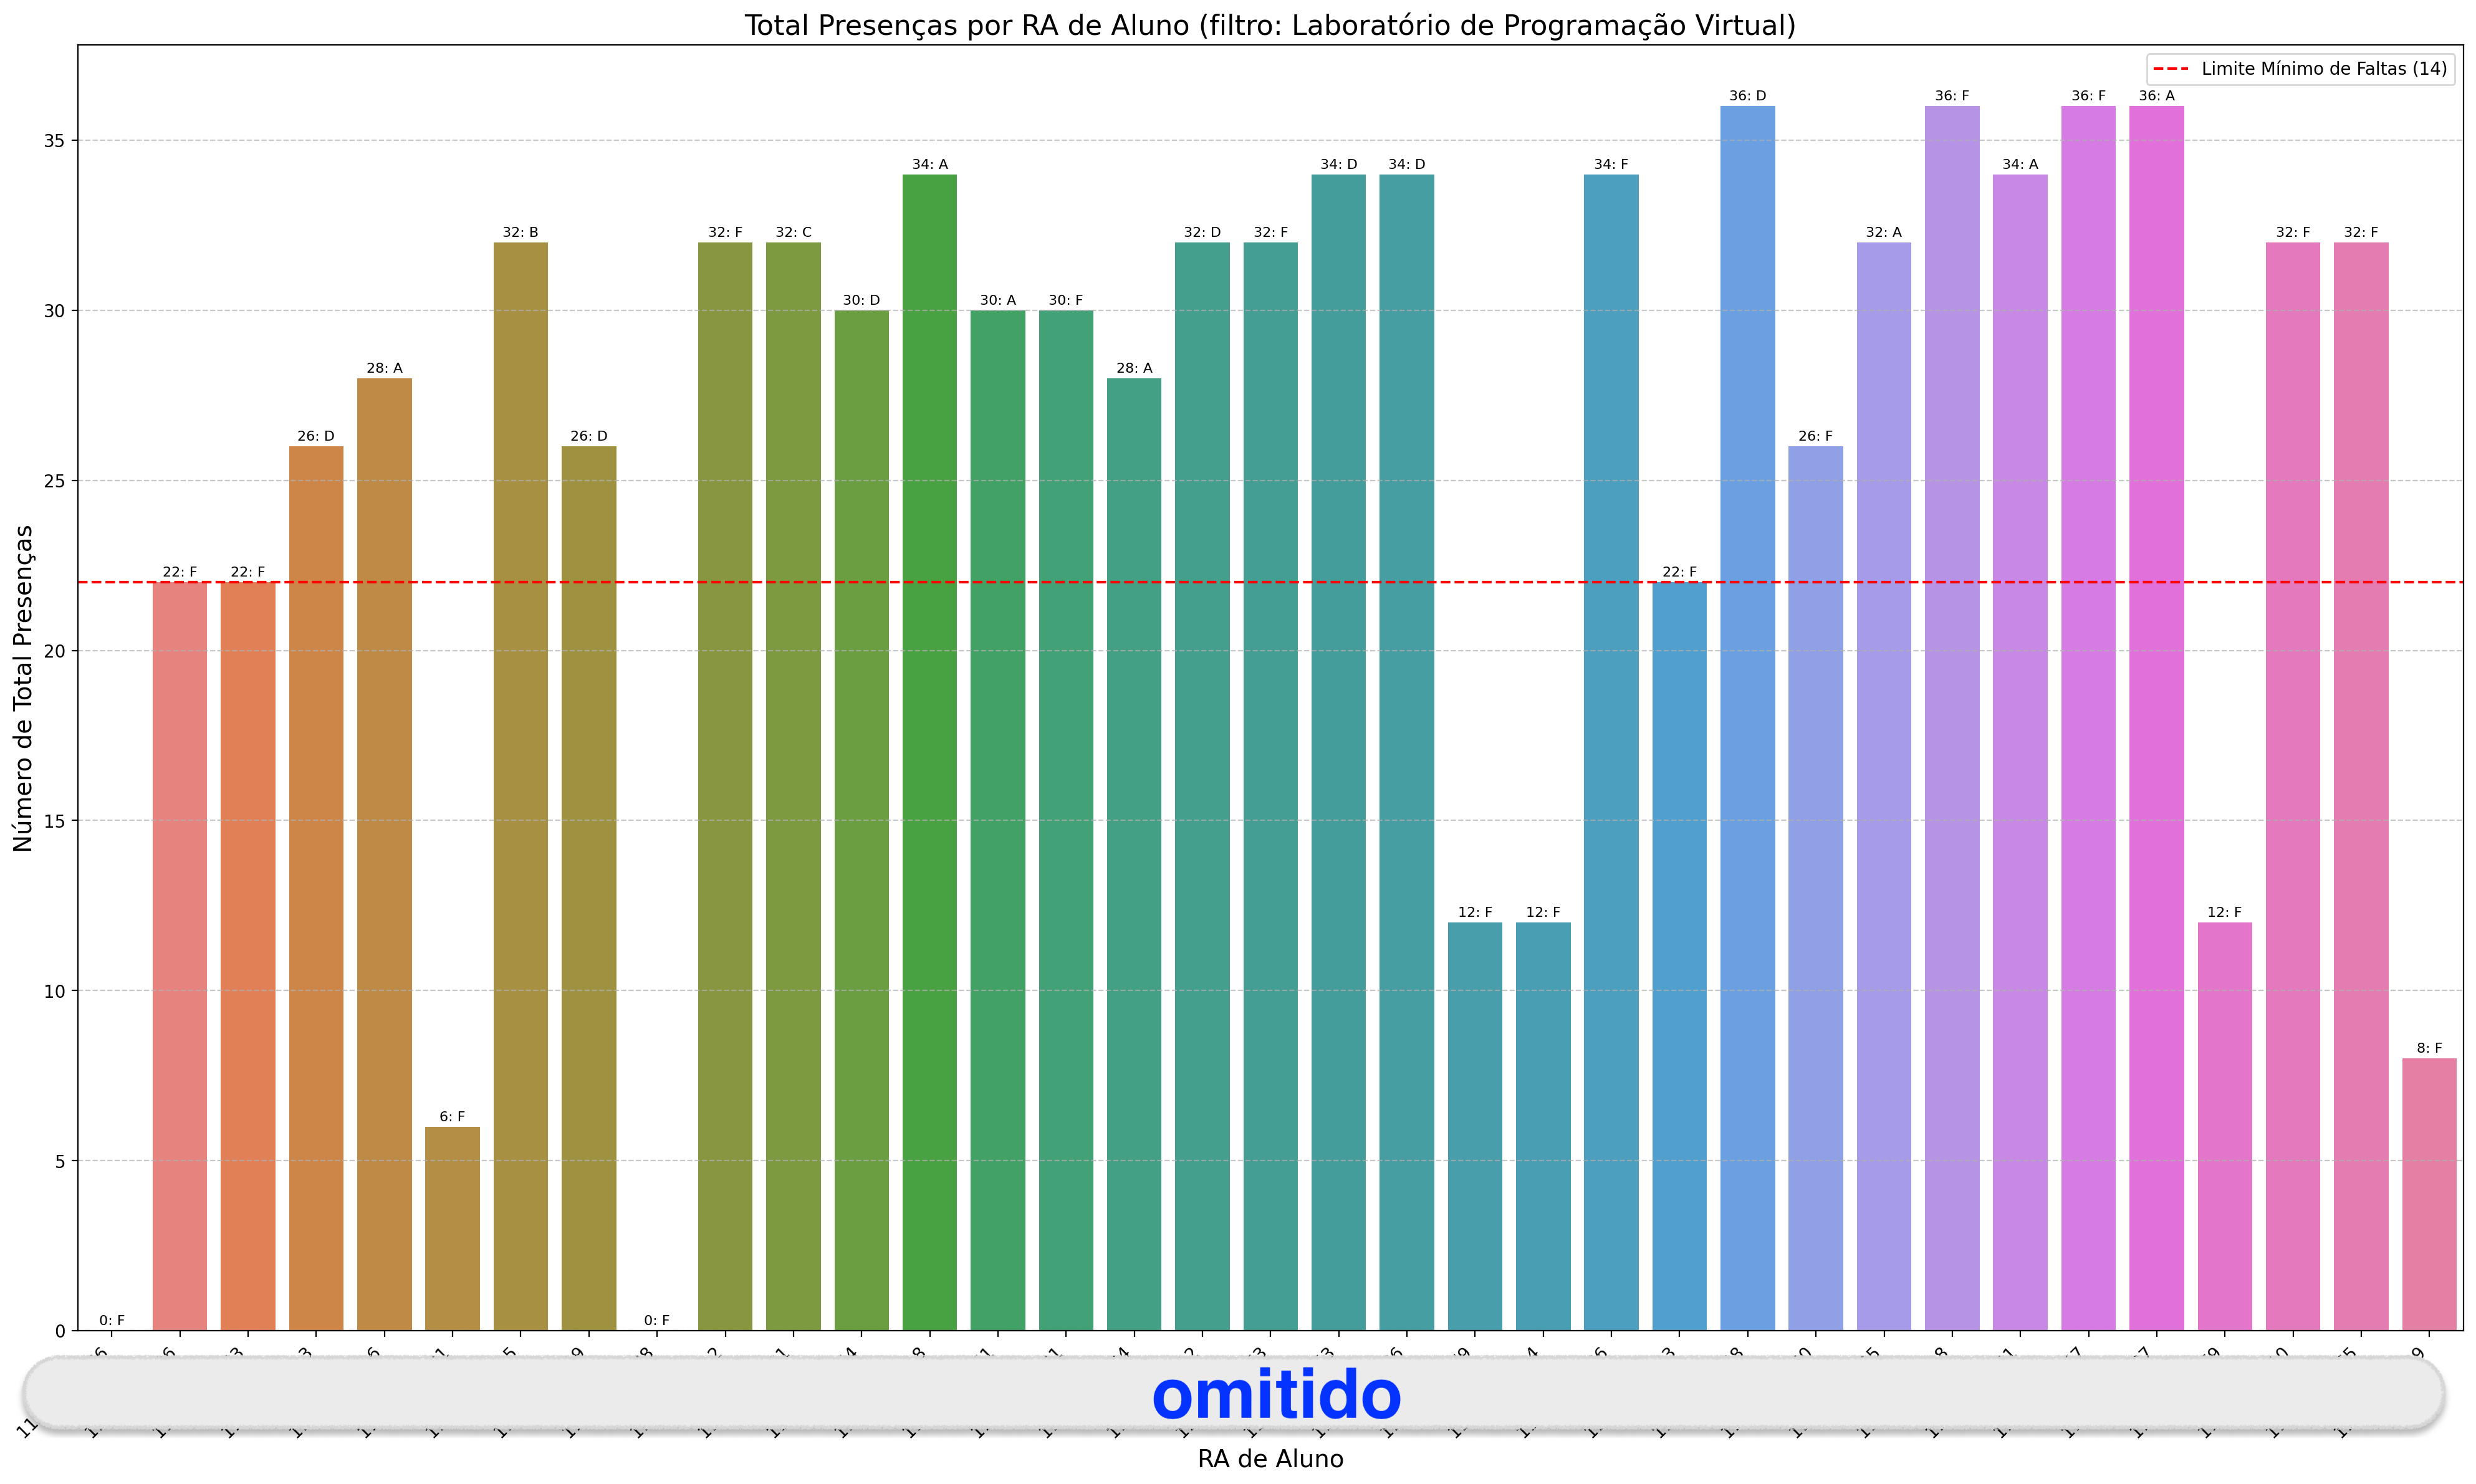
\includegraphics[width=0.96\textheight]{ApeA_alunos_Total_Presencas_RA.png}}
%     \caption{Gráfico contendo as presenças dos estudantes da turma B.}
%     \label{fig:ApeA_alunos_Total_Presencas_RA}
% \end{figure}

% \begin{figure}[!ht]
%     \centering
%     \rotatebox{270}{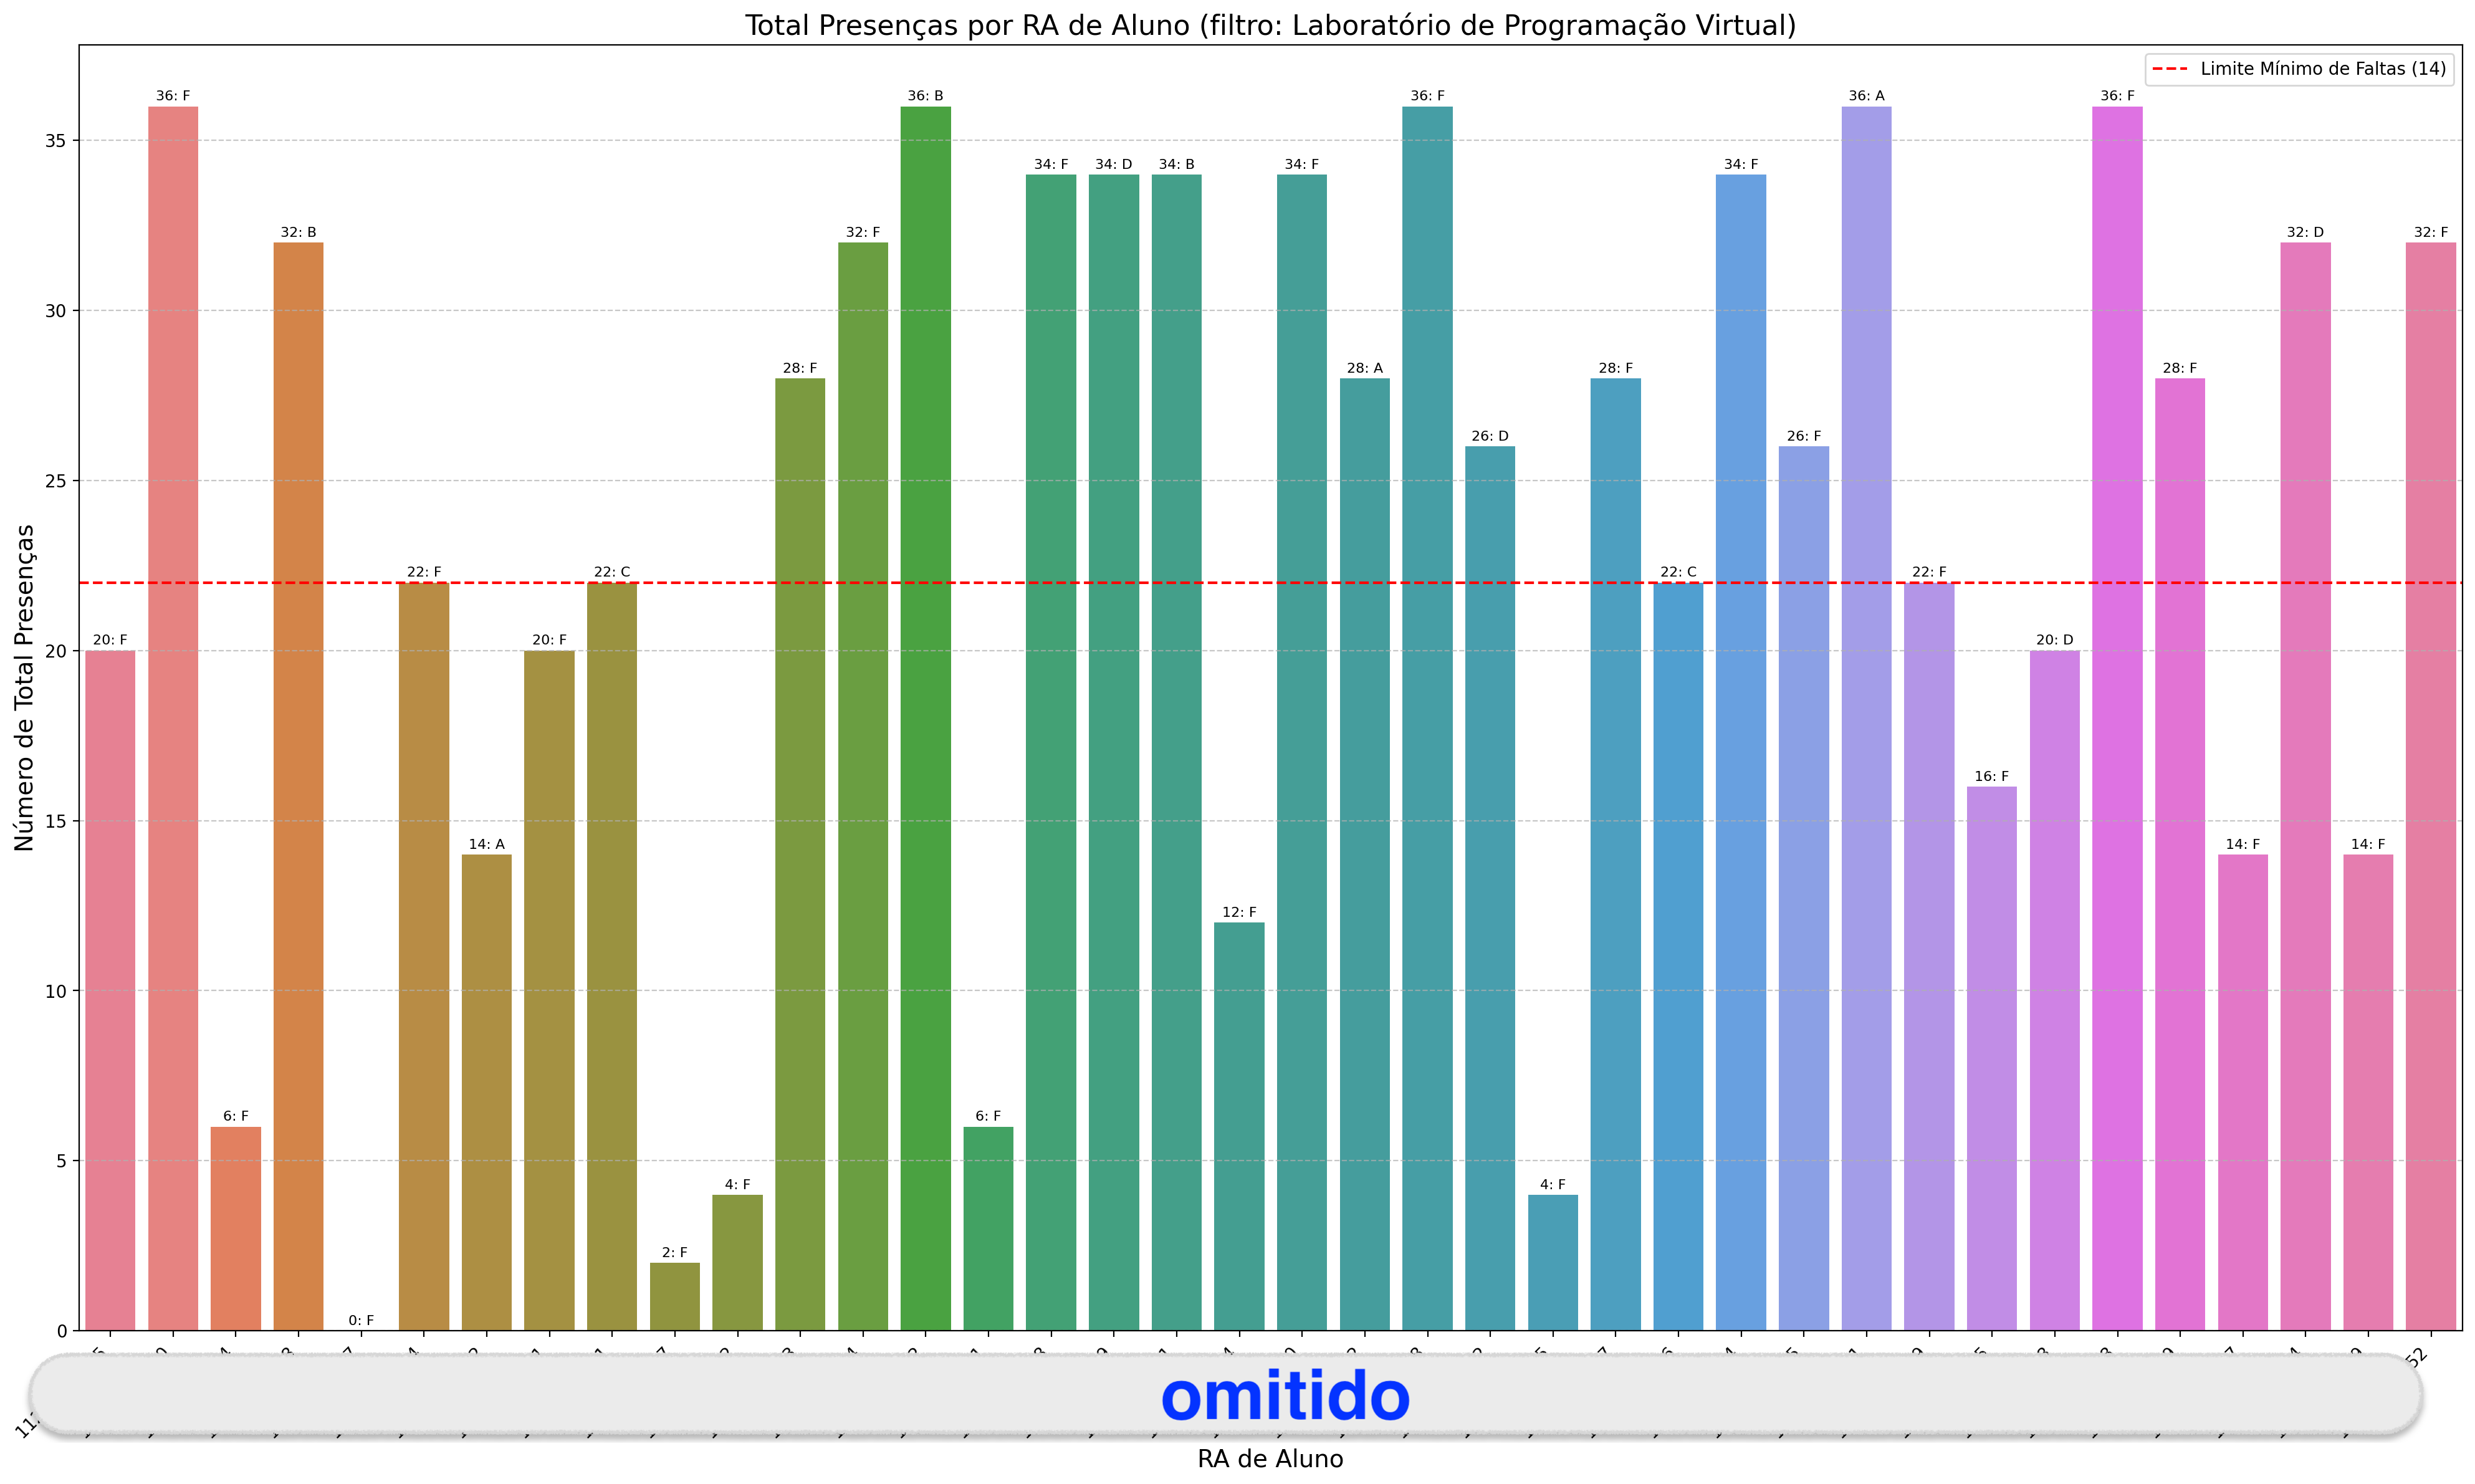
\includegraphics[width=0.96\textheight]{ApeA_alunos_Total_Presencas_RA_Turma_A.png}}
%     \caption{Gráfico contendo as presenças dos estudantes da turma A.}
%     \label{fig:ApeA_alunos_Total_Presencas_RA_Turma_A}
% \end{figure}



\subsection{Acessos no Moodle}

A Figura \ref{fig:ApeA_alunos_Acessos_Sem_Filtros_RA_turmaA} apresenta a imagem \verb|alunos_Acessos_Sem_Filtros_RA.png| contendo informa\-ções bastante relevantes, destacadas na área sombreada em vermelho, que correspondem ao número de acessos dos estudantes fora do horário das aulas na turma A. Esses dados sugerem uma possível falta de dedicação por parte dos estudantes nesta disciplina ao longo do período regular até a prova final. No topo de cada barra, são exibidos os totais de acessos, juntamente com o conceito atribuído ao estudante antes do exame final (sendo permitido realizar o exame final apenas para os estudantes com conceitos D e F). Um gráfico semelhante para a turma B é apresentado na Figura \ref{fig:ApeA_alunos_Acessos_Sem_Filtros_RA_turmaB}.

\begin{figure}[!ht]
    \centering
    \rotatebox{270}{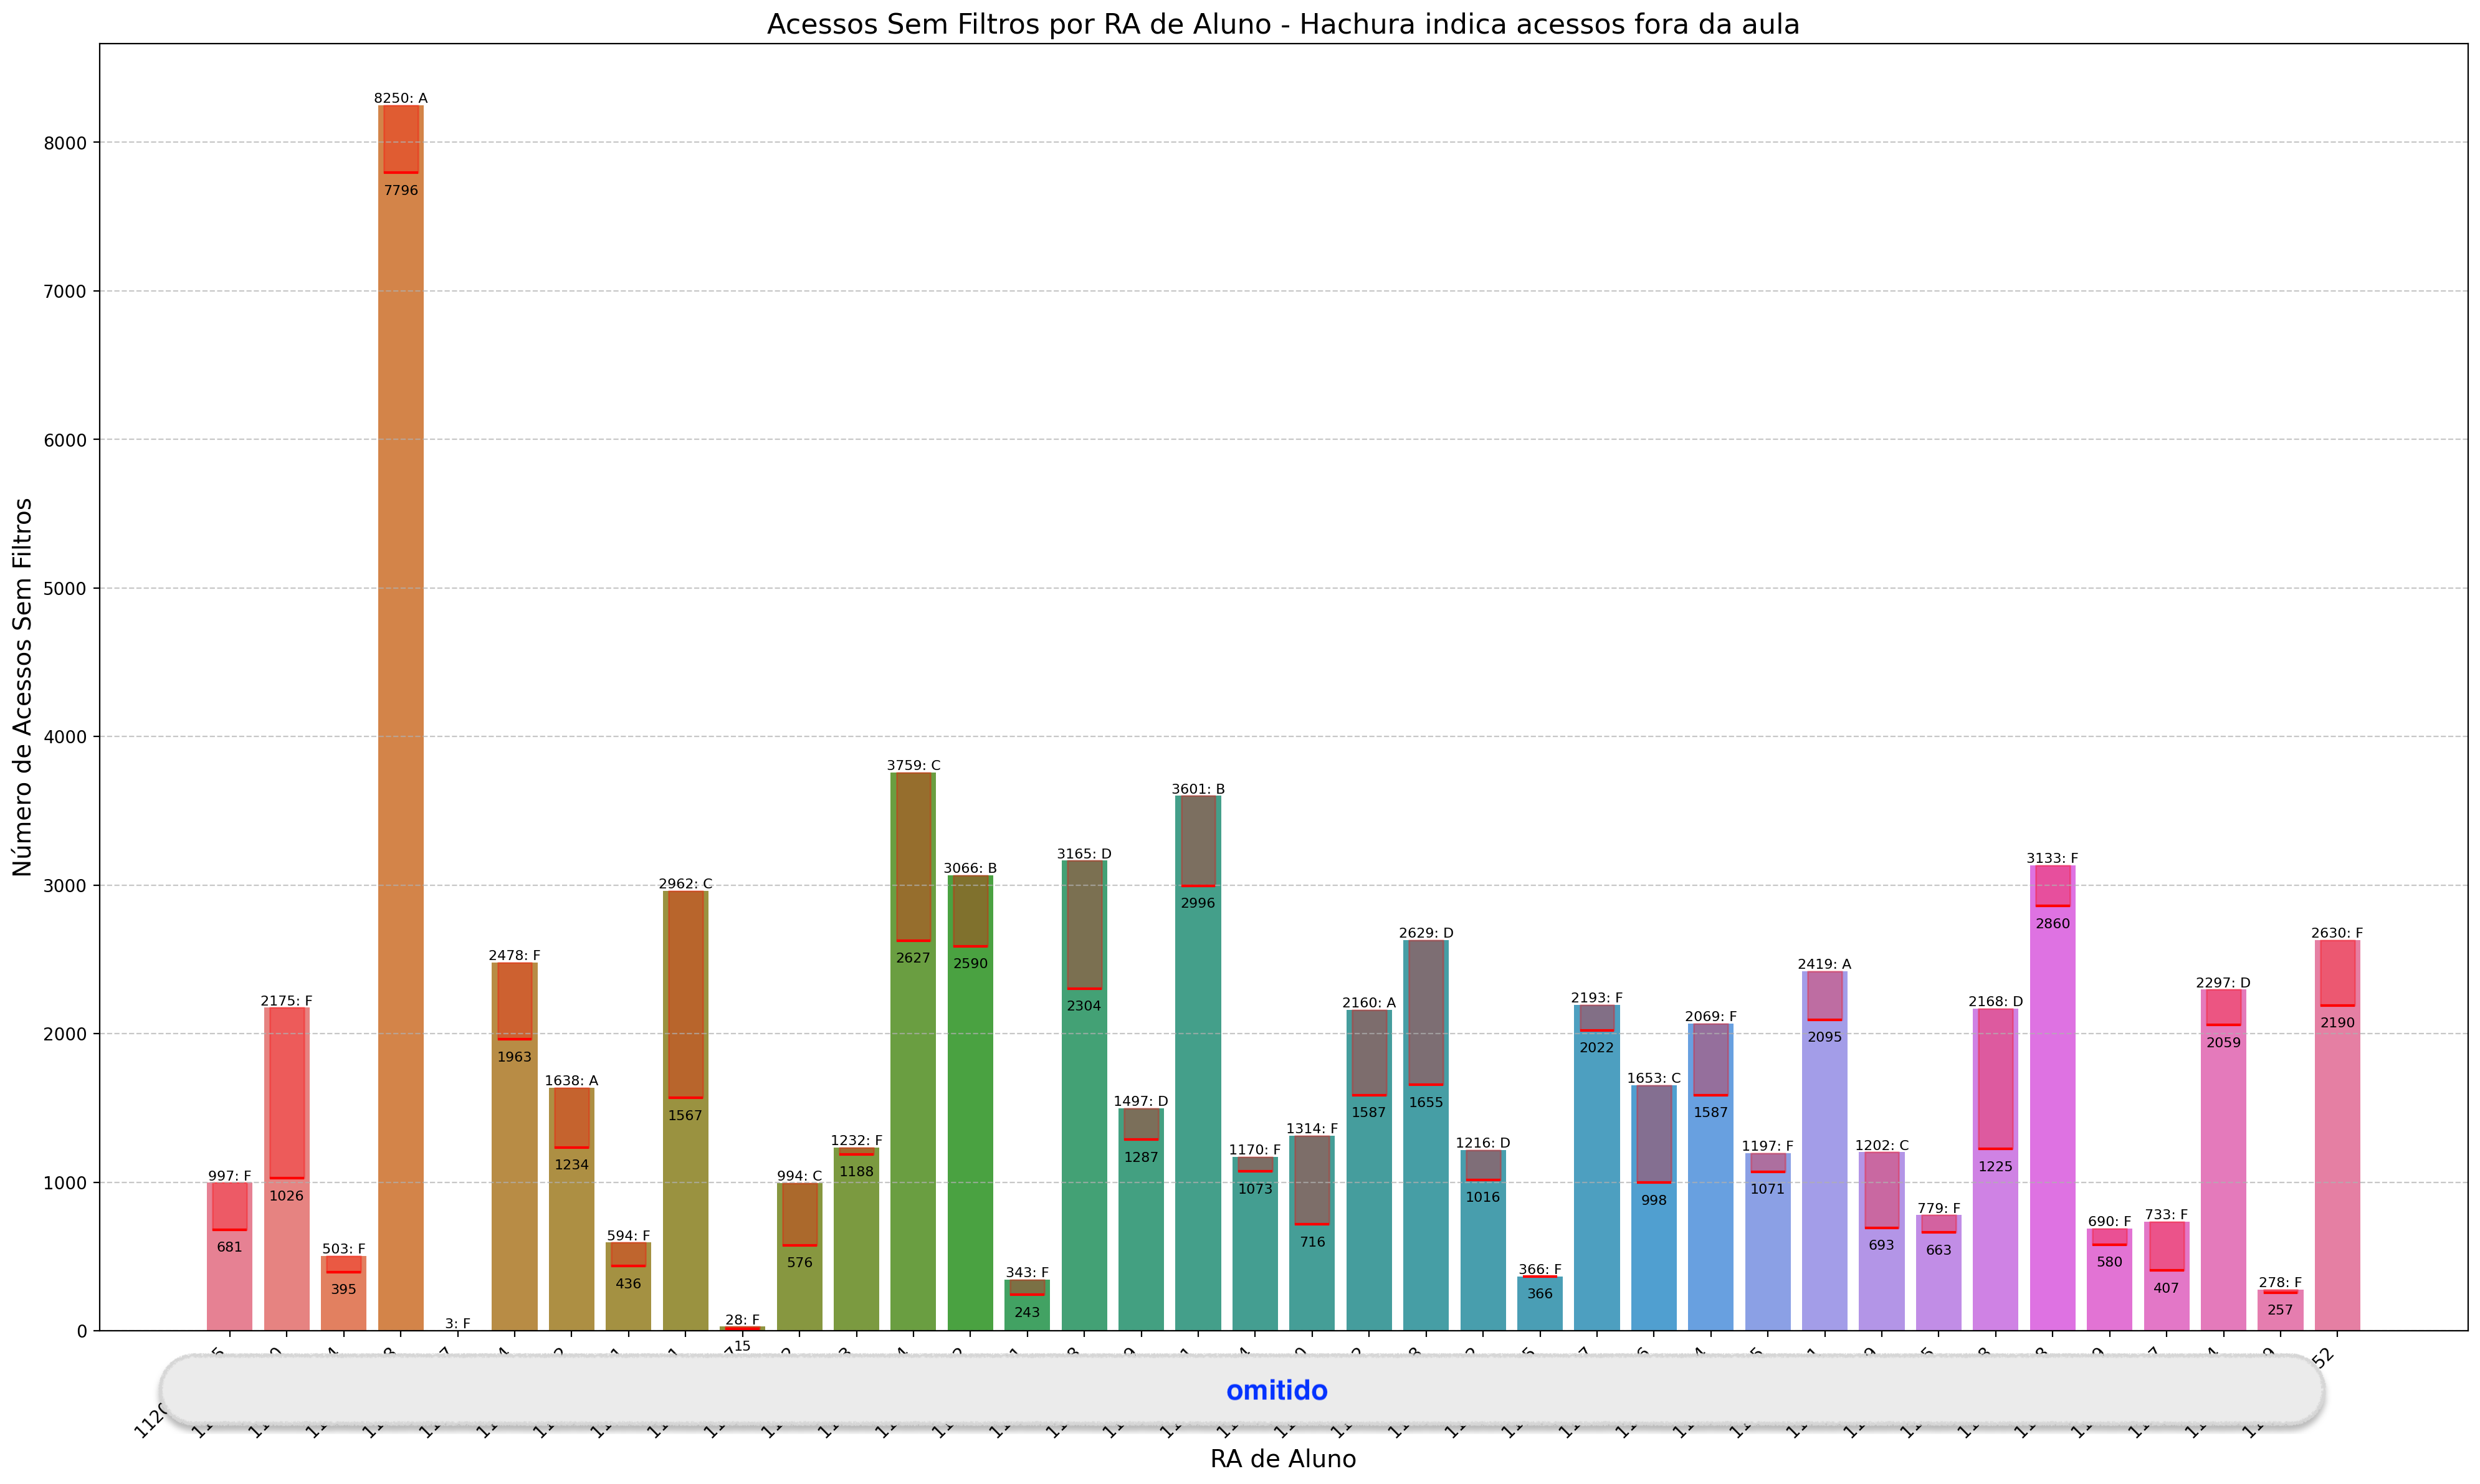
\includegraphics[width=0.96\textheight]{ApeA_alunos_Acessos_Sem_Filtros_RA_turmaA.png}}
    \caption{Gráfico contendo os acessos totais dos estudantes da turma A, com destaque para o baixo acesso fora da aula.}
    \label{fig:ApeA_alunos_Acessos_Sem_Filtros_RA_turmaA}
\end{figure}

\begin{figure}[!ht]
    \centering
    \rotatebox{270}{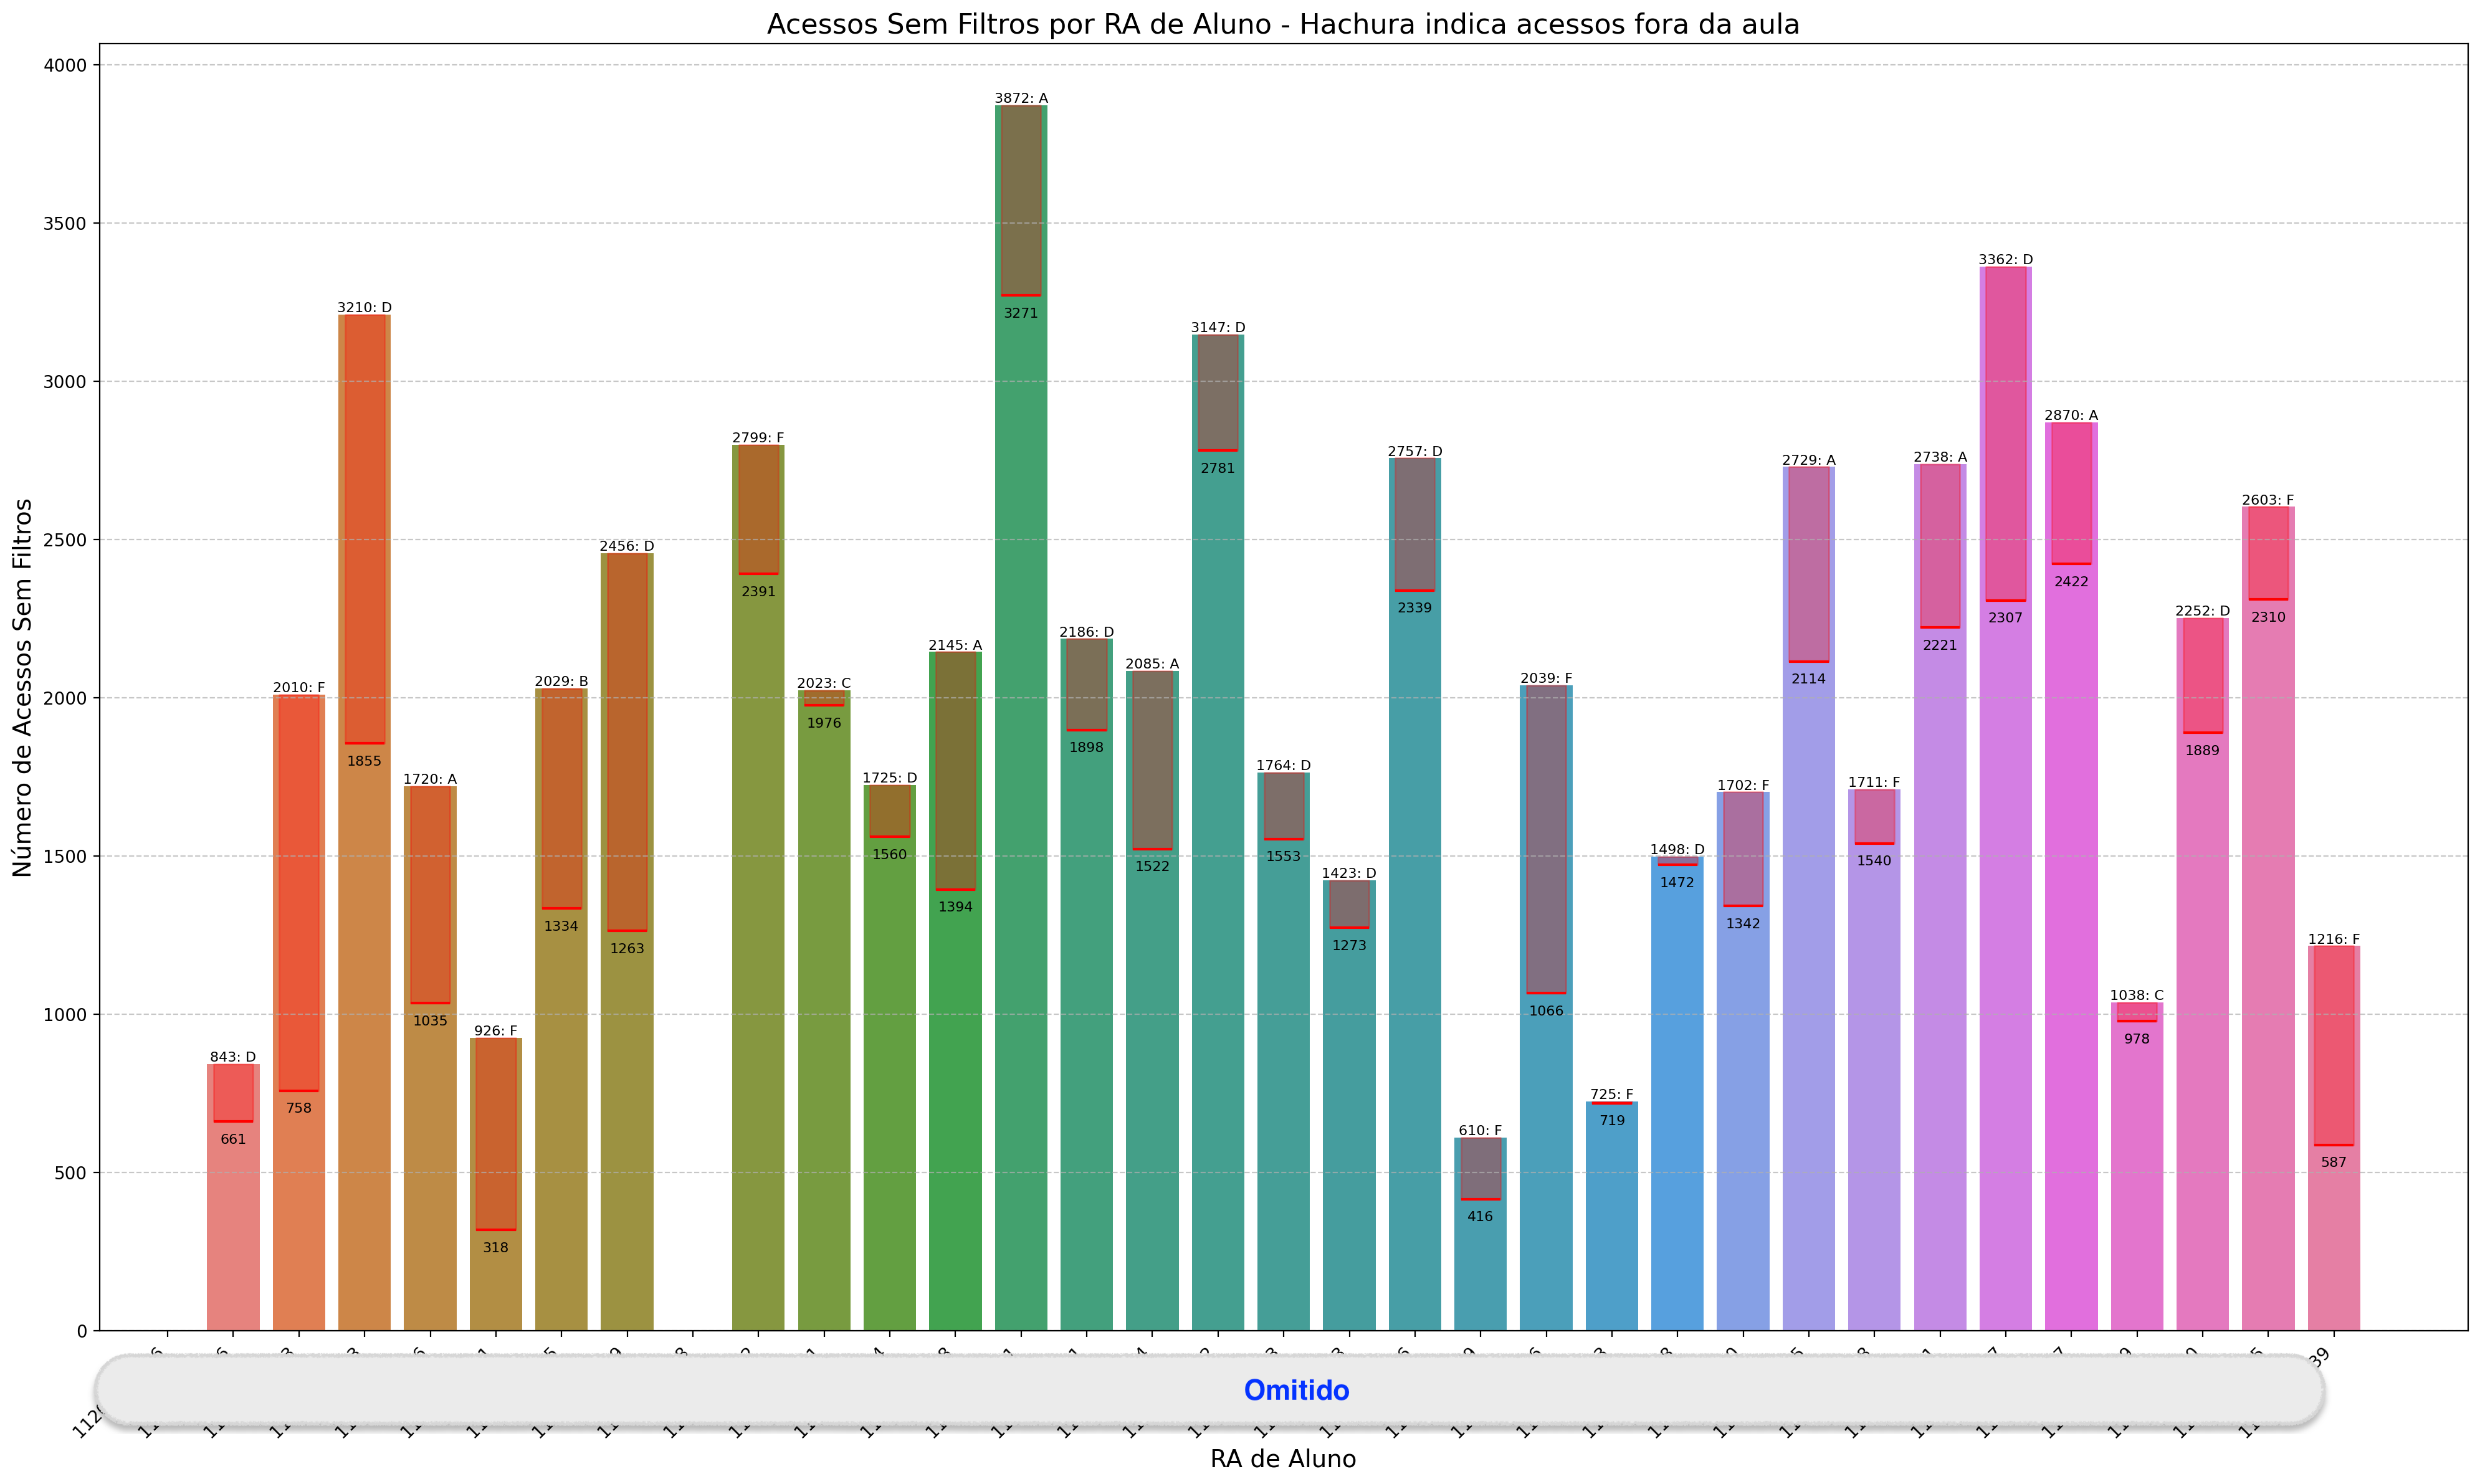
\includegraphics[width=0.96\textheight]{ApeA_alunos_Acessos_Sem_Filtros_RA_turmaB.png}}
    \caption{Gráfico contendo os acessos totais dos estudantes da turma B, com destaque para o baixo acesso fora da aula.}
    \label{fig:ApeA_alunos_Acessos_Sem_Filtros_RA_turmaA}
\end{figure}

\section{Acessos às atividades do Moodle}

O gráfico de barras da Figura \ref{fig:ApeA_Acessos_EPs} apresenta o número de estudantes que tentaram resolver cada um dos 80 EPs, distribuídos ao longo do eixo \( x \). No eixo \( y \), está representado o número de estudantes que tentaram realizar cada EP. Cada barra no gráfico corresponde a um EP específico, como ``EP1\_1'', ``EP1\_2'', ..., ``EP6\_23''. Observa-se uma variação considerável no número de acessos entre os diferentes EPs, indicando diferentes níveis de interação dos estudantes com o material disponibilizado. Além disso, o gráfico inclui uma linha de tendência exponencial com um coeficiente de determinação \( R^2=0.449 \), indicando que a linha é uma aproximação moderada para os dados. Esta linha ajuda a visualizar a tendência geral de decrescimento dos acessos ao longo dos EPs. Isso pode indicar o baixo desempenho dos estudantes na prova final, como relatado na próxima seção. A cor azul tem os EPs relacionados à primeira prova. A cor verde é associada aos EPs relacionados a vetores, enquanto a cor salmão representa os EPs relacionados a matrizes, ambas abordando o conteúdo da prova final. Finalmente, vale enfatizar ainda que aproximadamente 60 destes EPs foram resolvidos em sala de aula pelo professor, com é possível observar os EPs que se aproximam da linha de tendência.

\begin{figure}[!ht]
    \centering
    \rotatebox{270}{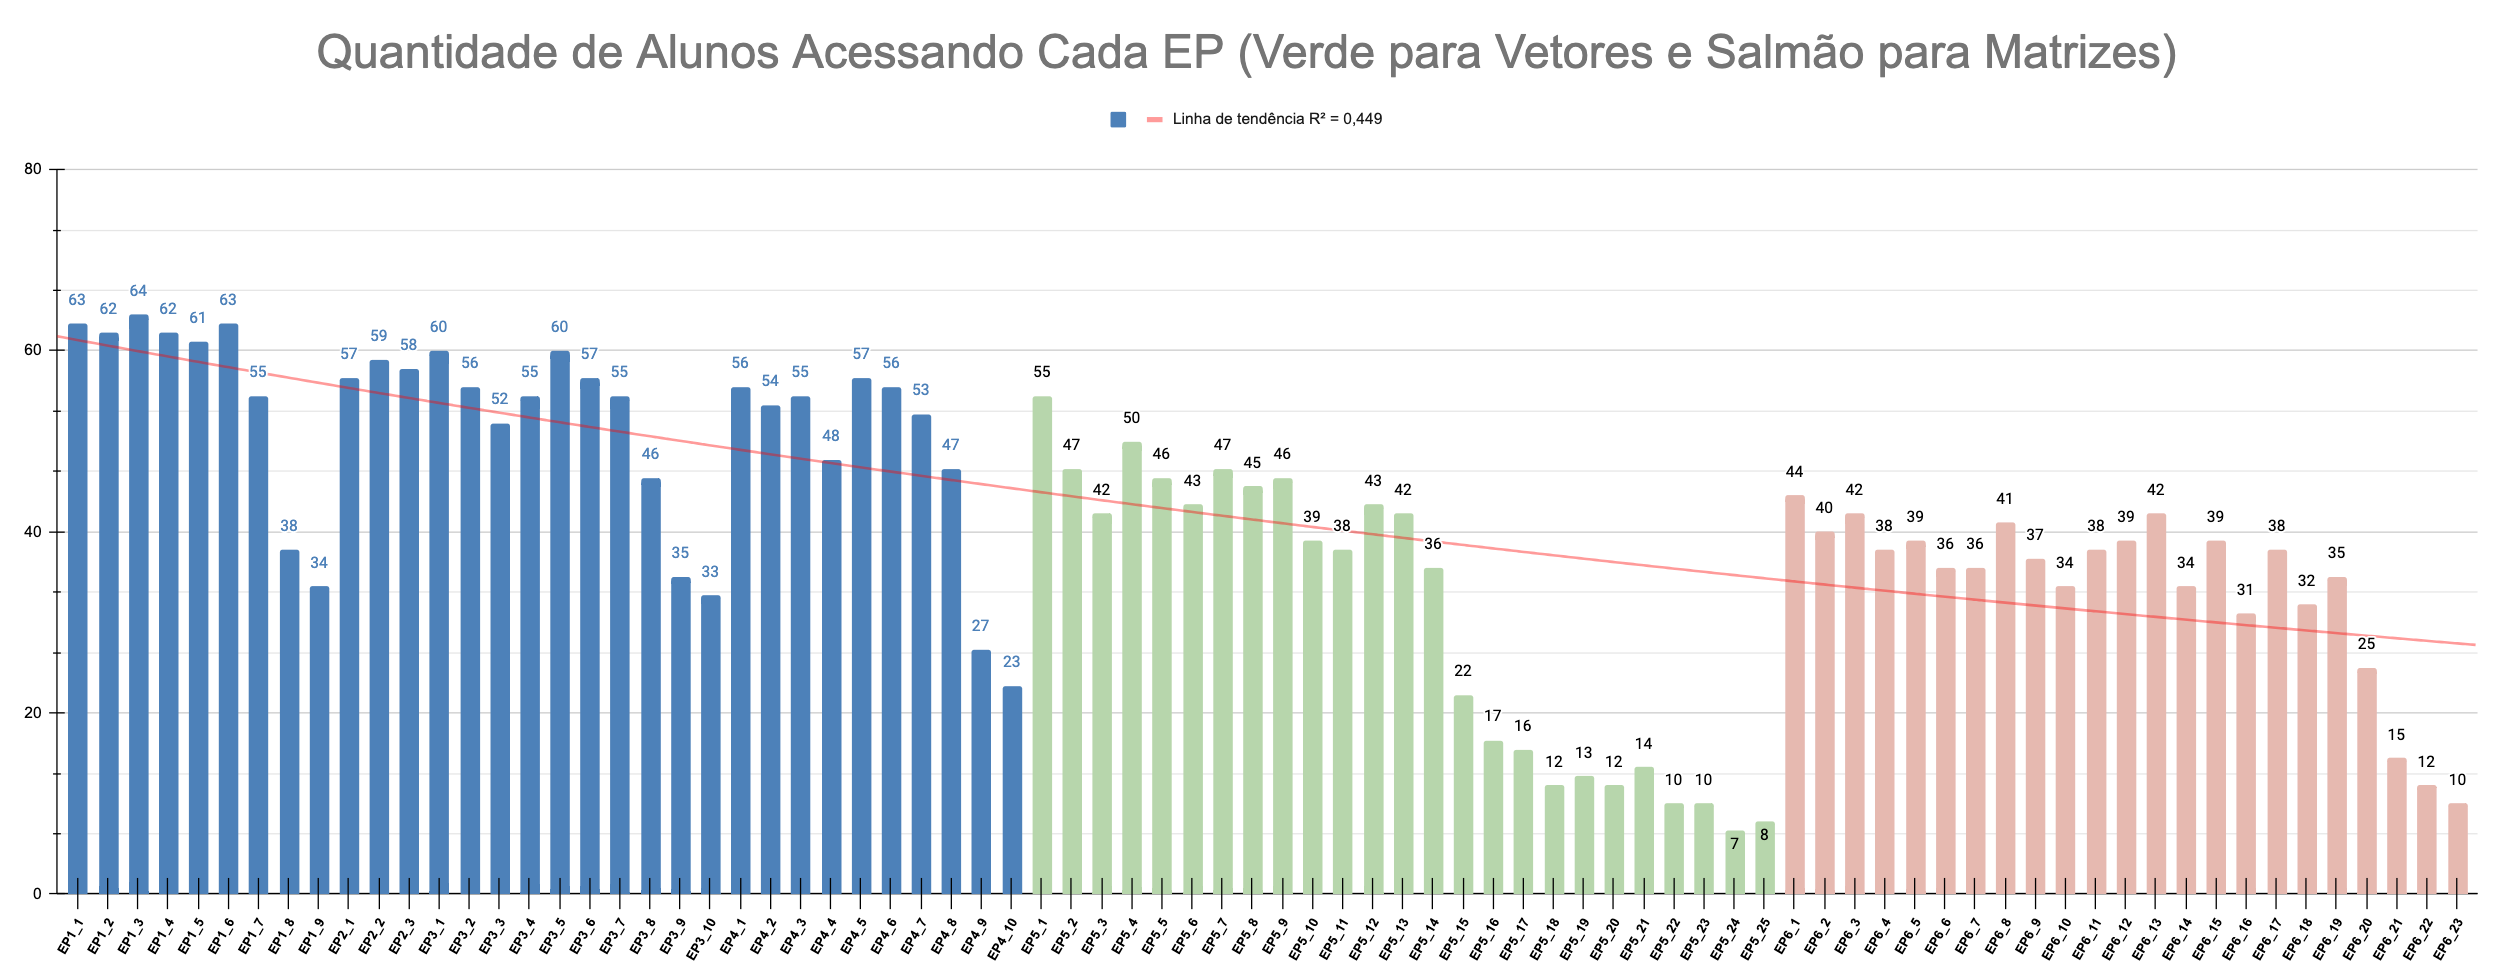
\includegraphics[width=0.96\textheight]{ApeA_Acessos_EPs.png}}
    \caption{Quantidade de estudantes que tentaram resolver os EP (verde para EPs sobre vetores e salmão para matrizes).}
    \label{fig:ApeA_Acessos_EPs}
\end{figure}




\section{Tabelas comparativas - turma A vs. turma B}

Esta seção destaca a comparação do desempenho entre as turmas A e B, tanto antes quanto após a prova de recuperação. Antes do exame, a turma B exibia uma correlação mais pronunciada entre acessos e conceitos, com uma maior proporção de estudantes alcançando o conceito A. 

\subsection{Comparações antes da prova de recuperação}

Após a análise da tabela comparativa antes da prova de recuperação (Tabela \ref{tab:antes-recuperacao}), observa-se que a turma B apresentou uma correlação ligeiramente maior entre acessos (durante a aula e fora também) e conceitos em comparação com a turma A. No entanto, a turma B obteve um número maior de estudantes com conceito A, indicando um desempenho global melhor em relação à turma B antes da prova de recuperação. Por outro lado, a turma B teve uma proporção maior de estudantes com conceitos D e F, sugerindo um desempenho mais baixo nesse período. Esses valores foram alterados após a prova de recuperação, como apresentado na próxima seção.

\begin{table}[htbp]
    \centering
    \caption{Tabela comparativa - antes da prova de recuperação}
    \label{tab:antes-recuperacao}
    \begin{tabular}{|c|c|c|c|c|c|c|c|c|}
      \hline
      \rowcolor[HTML]{EFEFEF} 
      & \multicolumn{2}{c|}{\cellcolor[HTML]{C0C0C0}\textbf{Correlações (desempenho vs)}} & \multicolumn{5}{c|}{\cellcolor[HTML]{C0C0C0}\textbf{Conceitos}} & \cellcolor[HTML]{C0C0C0}\textbf{Reprovação} \\
      \cline{2-3} \cline{4-8} \cline{9-9}
      \rowcolor[HTML]{EFEFEF} 
      \textbf{Turma} & \textbf{Acessos} & \textbf{Presenças} & \textbf{A} & \textbf{B} & \textbf{C} & \textbf{D} & \textbf{F} & \textbf{\%} \\
      \hline
      A & 0.498 & 0.389 & 3 & 3 & 2 & 4 & 26 & 68.42 \\
      \hline
      B & 0.558 & 0.526 & 7 & 1 & 1 & 7 & 19 & 54.29 \\
      \hline
    \end{tabular}
\end{table}

\subsection{Comparações após a prova de recuperação - resultado final}


Após a realização da prova de recuperação e a obtenção dos resultados finais, conforme apresentado na tabela comparativa (Tabela \ref{tab:apos-recuperacao}), notamos que houve uma melhoria no desempenho da turma A, com um aumento no número de estudantes com conceitos A, C e D e uma redução na proporção de estudantes com conceito F. Por outro lado, na turma B, embora não tenha alterado no número de estudantes com conceito A e B, houve também um aumento no número de estudantes com conceitos C e D. Porém, o destaque continua sendo a porcentagem de reprovações elevada na turma A (55.26\%) comparada à turma B (35.29\%). Nessa tabela não foram apresentadas as correlações entre desempenho e acessos (além de frequência), pois não foi mais contabilizada a presença após a prova 2, visto que alguns estudantes que já foram aprovados não participaram mais das aulas.

\begin{table}[htbp]
    \centering
    \caption{Tabela comparativa - após da prova de recuperação}
    \label{tab:apos-recuperacao}
    \begin{tabular}{|c|c|c|c|c|c|c|}
      \hline
      \rowcolor[HTML]{EFEFEF} 
       & \multicolumn{5}{c|}{\cellcolor[HTML]{C0C0C0}\textbf{Conceitos}} & \cellcolor[HTML]{C0C0C0}\textbf{Reprovação} \\
      \cline{2-6} \cline{7-7}
      \rowcolor[HTML]{EFEFEF} 
      \textbf{Turma} & \textbf{A} & \textbf{B} & \textbf{C} & \textbf{D} & \textbf{F} & \textbf{\%} \\
      \hline
      A & 4 & 2 & 5 & 6 & 21 & 55.26 \\
      \hline
      B & 7 & 1 & 2 & 12 & 12 & 35.29 \\
      \hline
    \end{tabular}
\end{table}

\section{Considerações finais}

O experimento realizado nas turmas A e B da disciplina de Processamento da Informação no primeiro quadrimestre de 2024 proporcionou informações valiosas sobre o engajamento e desempenho dos estudantes. A análise dos dados de acesso ao Moodle, combinada com os conceitos obtidos, permitiu avaliar a correlação entre essas métricas e identificar áreas de melhoria.

Os resultados revelaram que a turma B apresentou uma correlação um pouco mais forte entre acessos, presenças e desempenho, com uma proporção maior de estudantes obtendo conceitos mais altos em geral. Isso sugere que, mesmo recebendo o mesmo conteúdo e avaliações semelhantes, uma turma pode ter um desempenho superior por razões que vão além do escopo deste estudo.
\
Após a prova de recuperação, observou-se uma melhoria geral no desempenho das turmas A e B, com mais estudantes alcançando conceitos superiores. 
%No entanto, a turma B também apresentou um aumento no número de estudantes com conceitos elevados, indicando uma variação positiva no desempenho dessa turma.

O serviço LabMoodle, desenvolvido para acompanhar as atividades dos estudantes no Moodle, demonstrou ser uma ferramenta valiosa para os professores. Ao fornecer informações detalhadas sobre acessos, presenças e desempenho, o serviço permitiu identificar pontos de atenção e orientar estratégias pedagógicas mais eficazes.

É importante ressaltar que os dados de acesso ao Moodle e as presenças em aula representam apenas uma parte do processo de aprendizagem dos estudantes. Outros fatores, como a dedicação individual fora do horário de aula, as estratégias de estudo e o engajamento com o conteúdo, também desempenham um papel crucial no desempenho acadêmico.

Uma limitação deste método é que alguns estudantes podem realizar seus estudos fora do Moodle, tanto durante a aula quanto fora dela. Além disso, não foi avaliado o conhecimento prévio dos estudantes. Assim, estudantes com experiência em programação podem não participar das atividades e ainda assim apresentar um bom desempenho, como observado nos gráficos apresentados. Finalmente, presume-se que os IPs de um laboratório devem ter um prefixo, como ``172.17.14'', conforme apresentado na Figura \ref{fig:ApeA_parte2}. O professor pode também considerar todos os IPs, substituindo o prefixo por ``172'' (conforme a rede local) ou simplesmente ``.''.

Como sugestões para trabalhos futuros, considerando que os estudantes adquirem conhecimentos básicos de lógica de programação no seu ingresso na graduação, durante a disciplina de Bases Computacionais da Ciência (CS0), geralmente ministrada utilizando a linguagem Python, propõe-se algumas modificações nas avaliações da disciplina de Processamento da Informação. Uma sugestão seria realizar a primeira prova abrangendo conceitos até laços de repetição ao final da semana 4, funcionando como uma revisão dos conteúdos abordados no curso CS0. Na semana 7, poderia ser aplicada uma prova sobre vetores, e na semana 11, uma prova sobre matrizes, distribuídas com pesos de avaliação de 30\%, 35\% e 35\%, respectivamente. Outra sugestão é substituir os testes adaptativos de múltipla escolha em papel por uma implementação similar no próprio ambiente Moodle. Ou ainda realizar simulados antes de cada avaliação, valendo um bônus de 5\% em cada um. Finalmente, um estudante sugeriu resolver mais EPs passo-a-passo pelo professor, além de mostrar soluções prontas e explicar.

As informações obtidas neste experimento podem ser utilizadas para aprimorar o planejamento e a condução de futuras ofertas da disciplina. Ajustes nas abordagens pedagógicas, incentivos ao engajamento e um acompanhamento mais próximo dos estudantes com dificuldades podem ser implementados com base nas lições aprendidas.
